\section{Frequency mode 08}
\label{FM08}

\subsection{Spectra}
\label{FM08:spectra}

\begin{figure}[ht]
    \centering
    \begin{subfigure}[b]{0.9545\textwidth}
        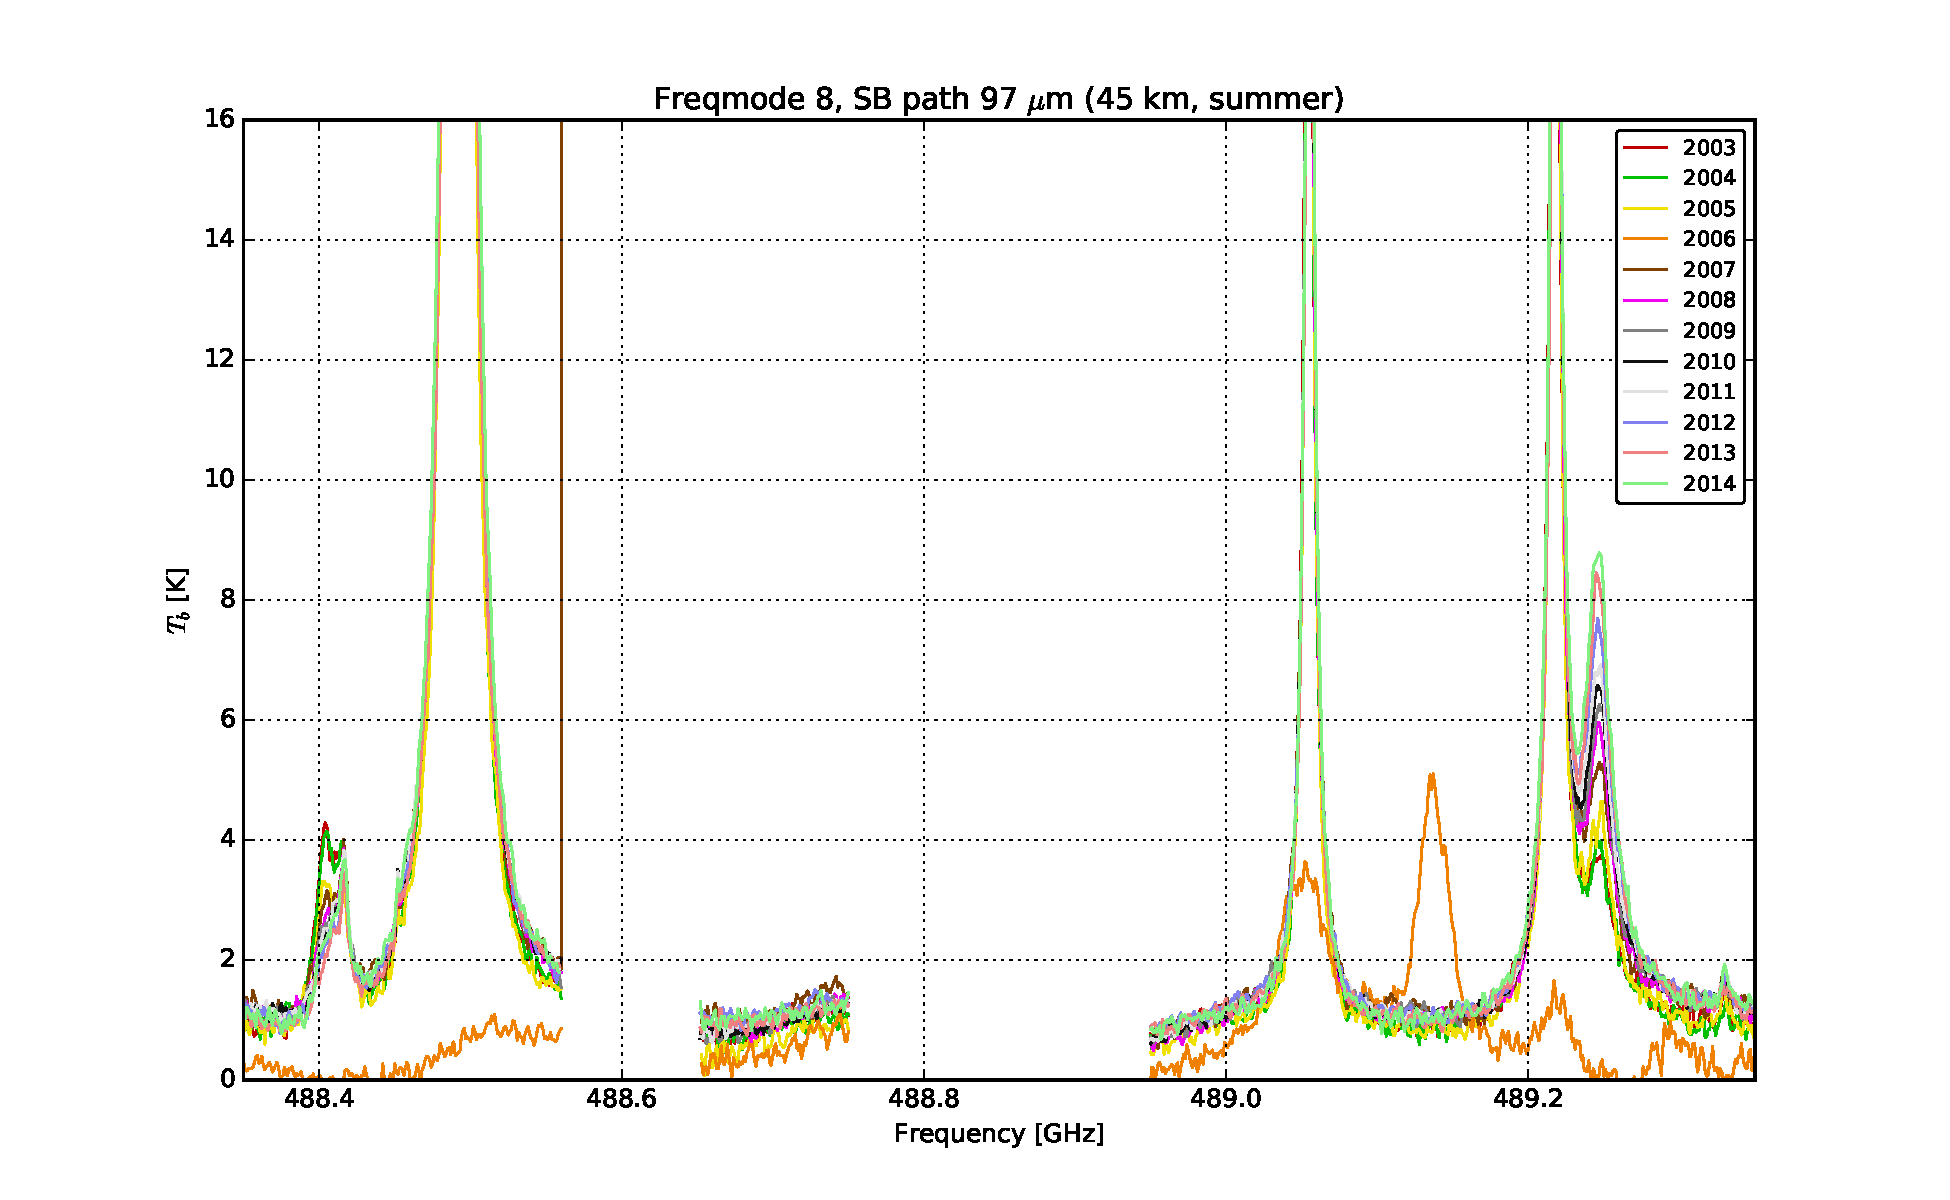
\includegraphics[width=\textwidth]{spectra/fm_08_spectra_summer_97u}
        \caption{summer}\label{fig:spectra:08:summer:97u}
    \end{subfigure}
    \begin{subfigure}[b]{0.9545\textwidth}
        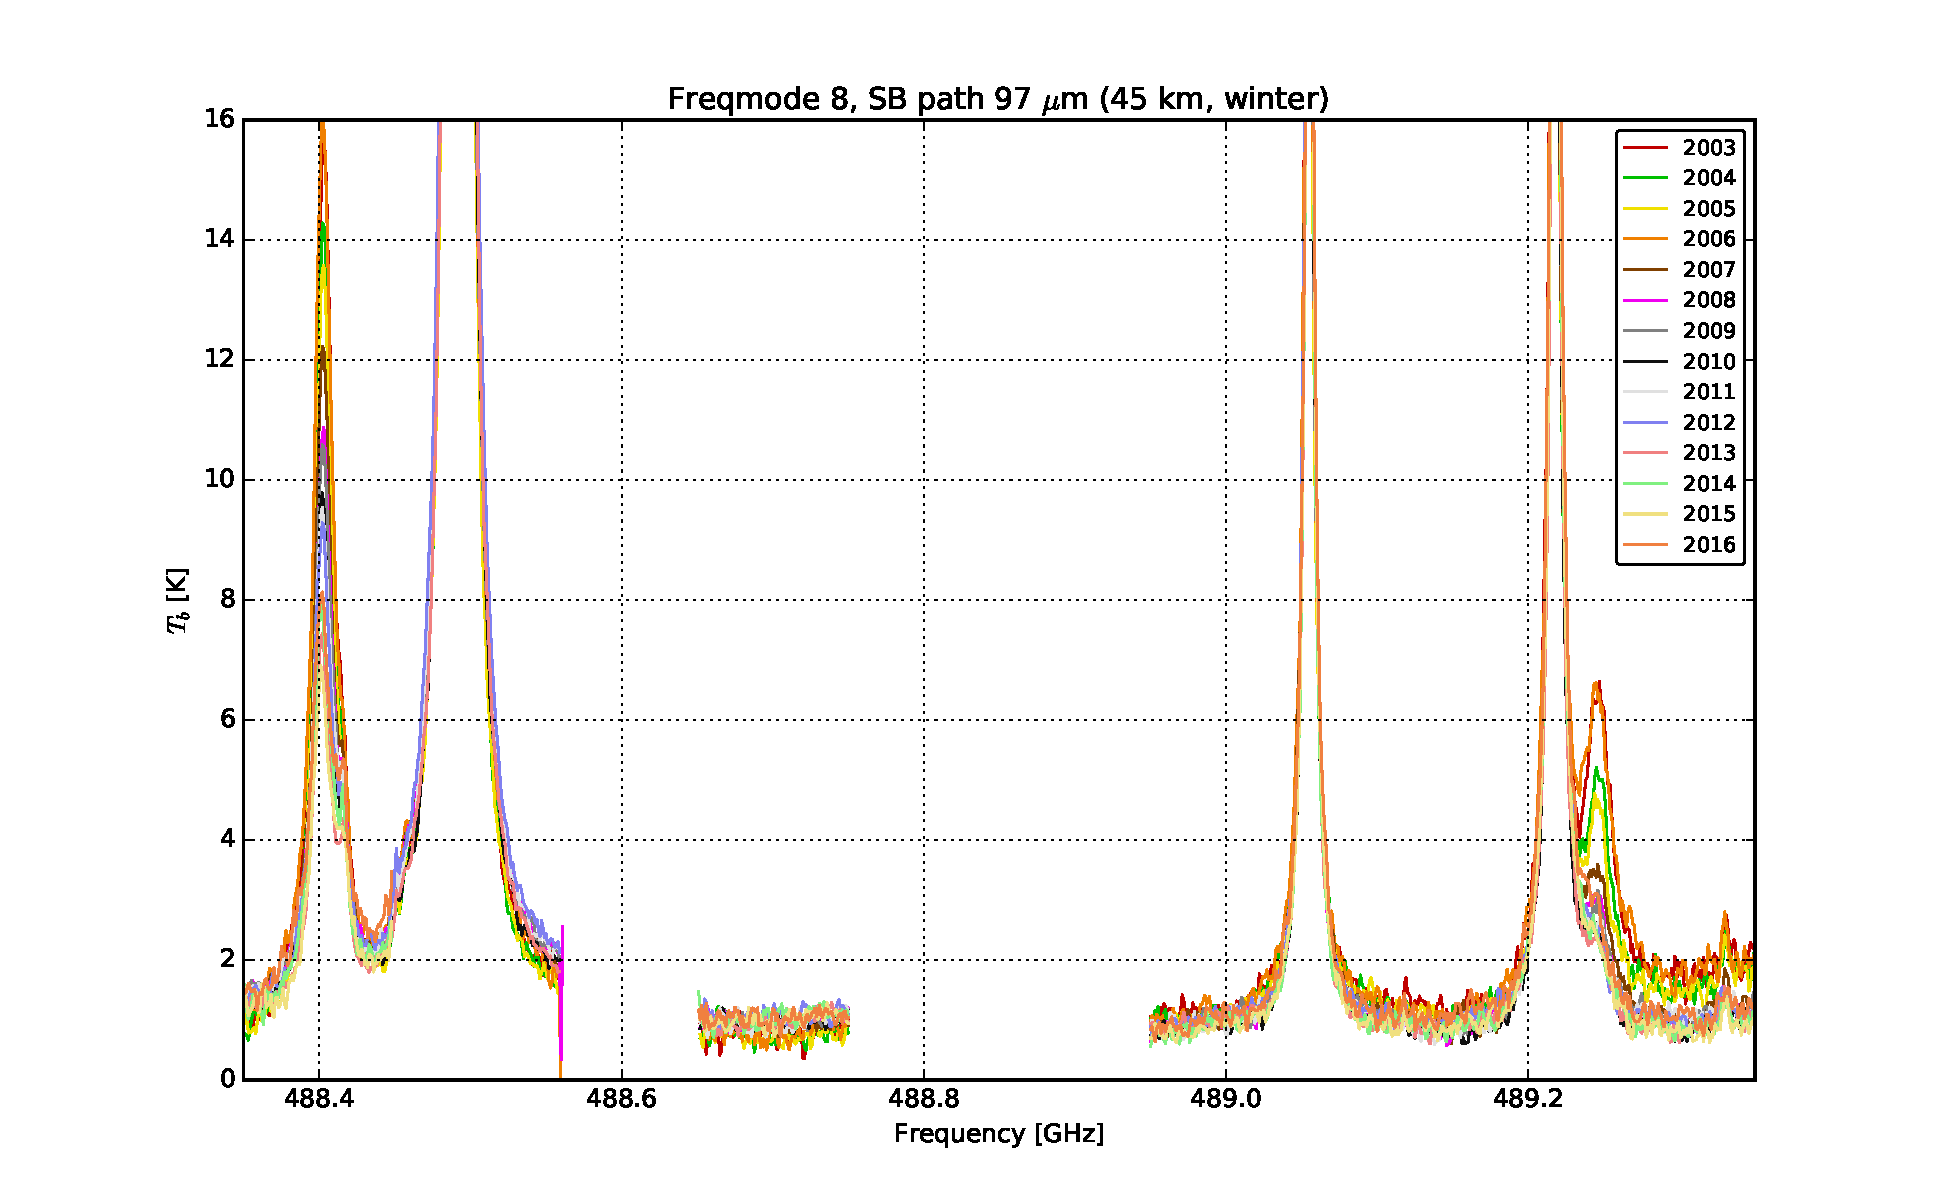
\includegraphics[width=\textwidth]{spectra/fm_08_spectra_winter_97u}
        \caption{winter}\label{fig:spectra:08:winter:97u}
    \end{subfigure}
    \caption{Annual median spectra for FM~08 for altitude interval 40--50~km at
        equatorial latitudes for the $97\,\mathrm{\mu m}$ sideband path. The
        unhealthy sub-bands~7 and~3 are between $\sim488.45$
        and~$488.65\,\mathrm{GHz}$.
        }\label{fig:spectra:08:97u}
\end{figure}

\begin{figure}[ht]
    \centering
    \begin{subfigure}[b]{0.9545\textwidth}
        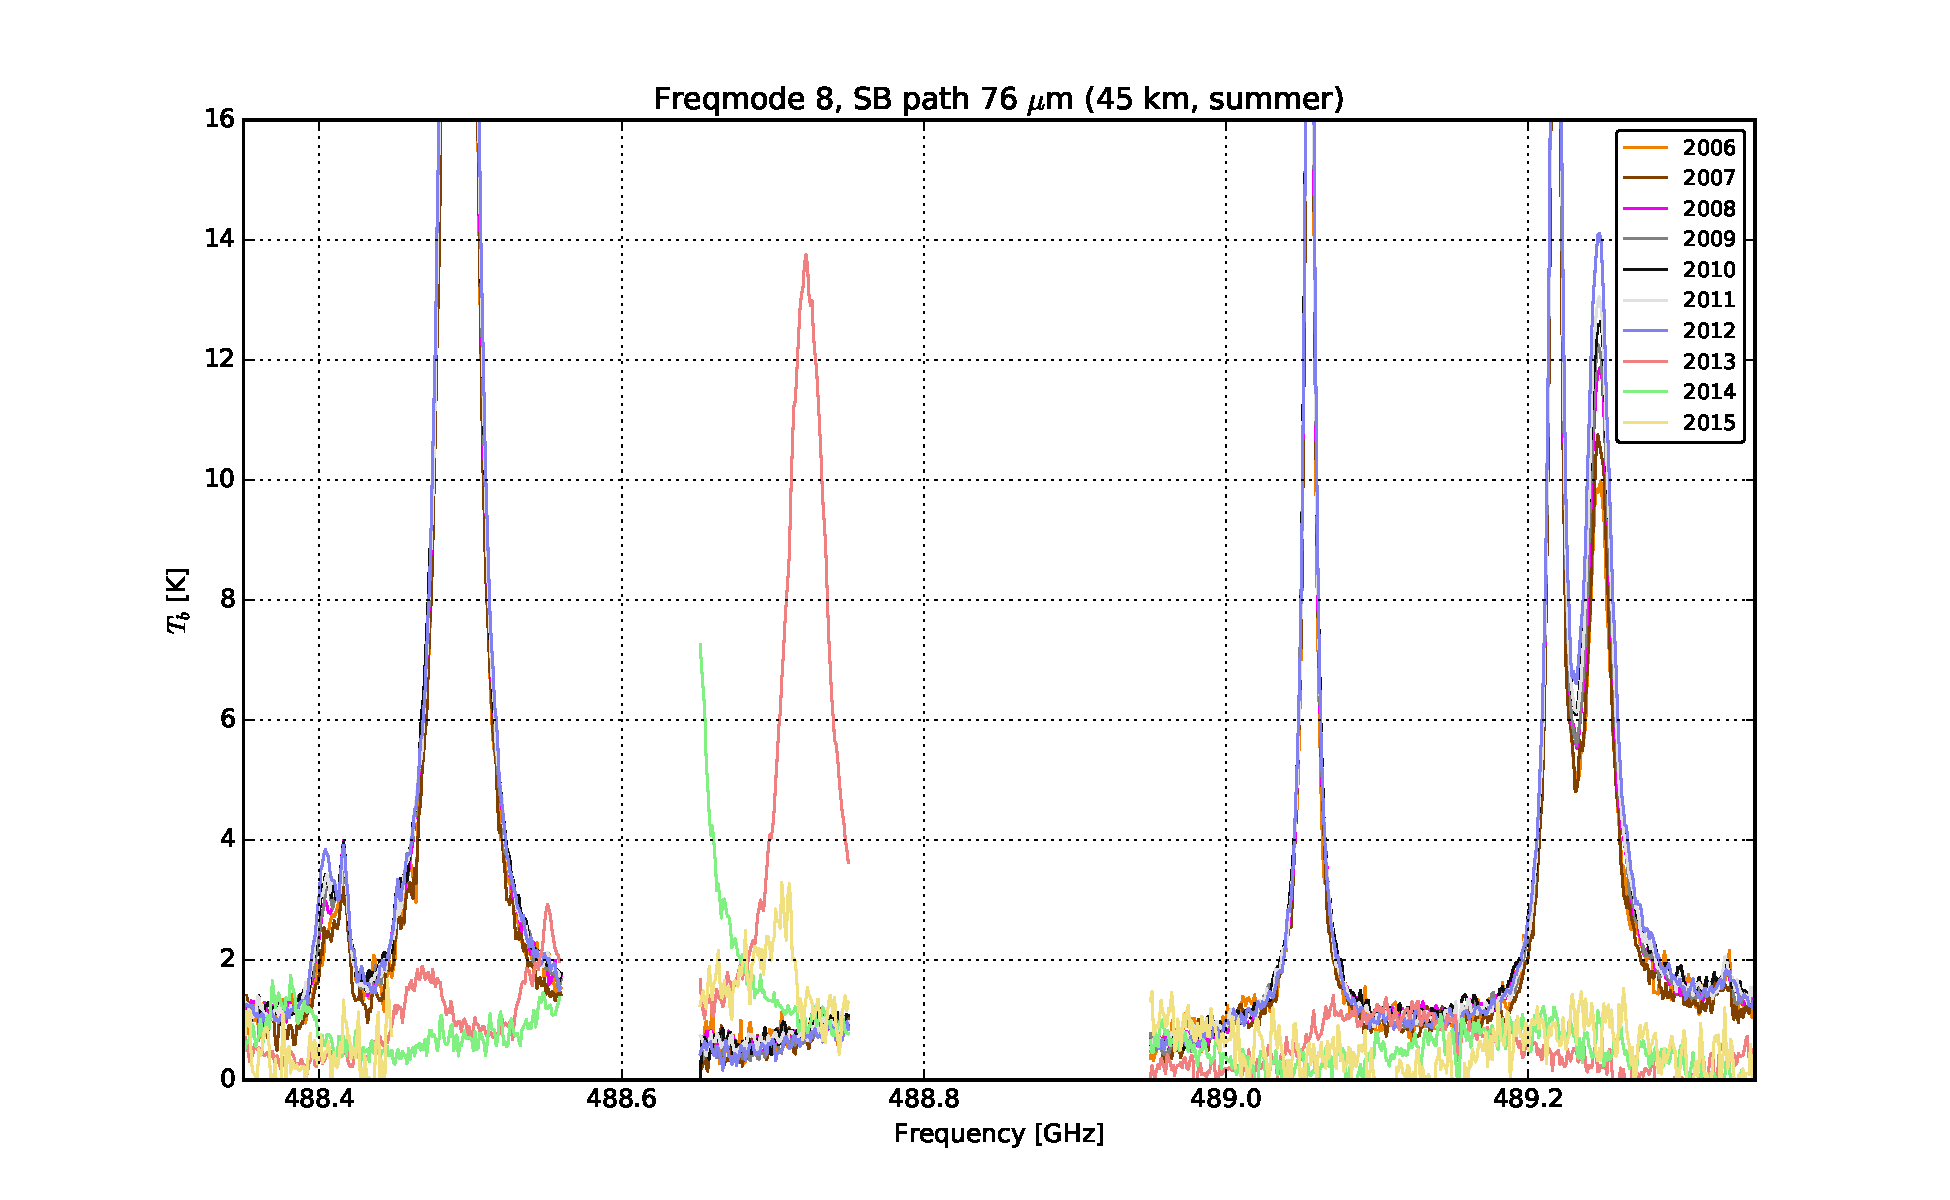
\includegraphics[width=\textwidth]{spectra/fm_08_spectra_summer_76u}
        \caption{summer}\label{fig:spectra:08:summer:76u}
    \end{subfigure}
    \begin{subfigure}[b]{0.9545\textwidth}
        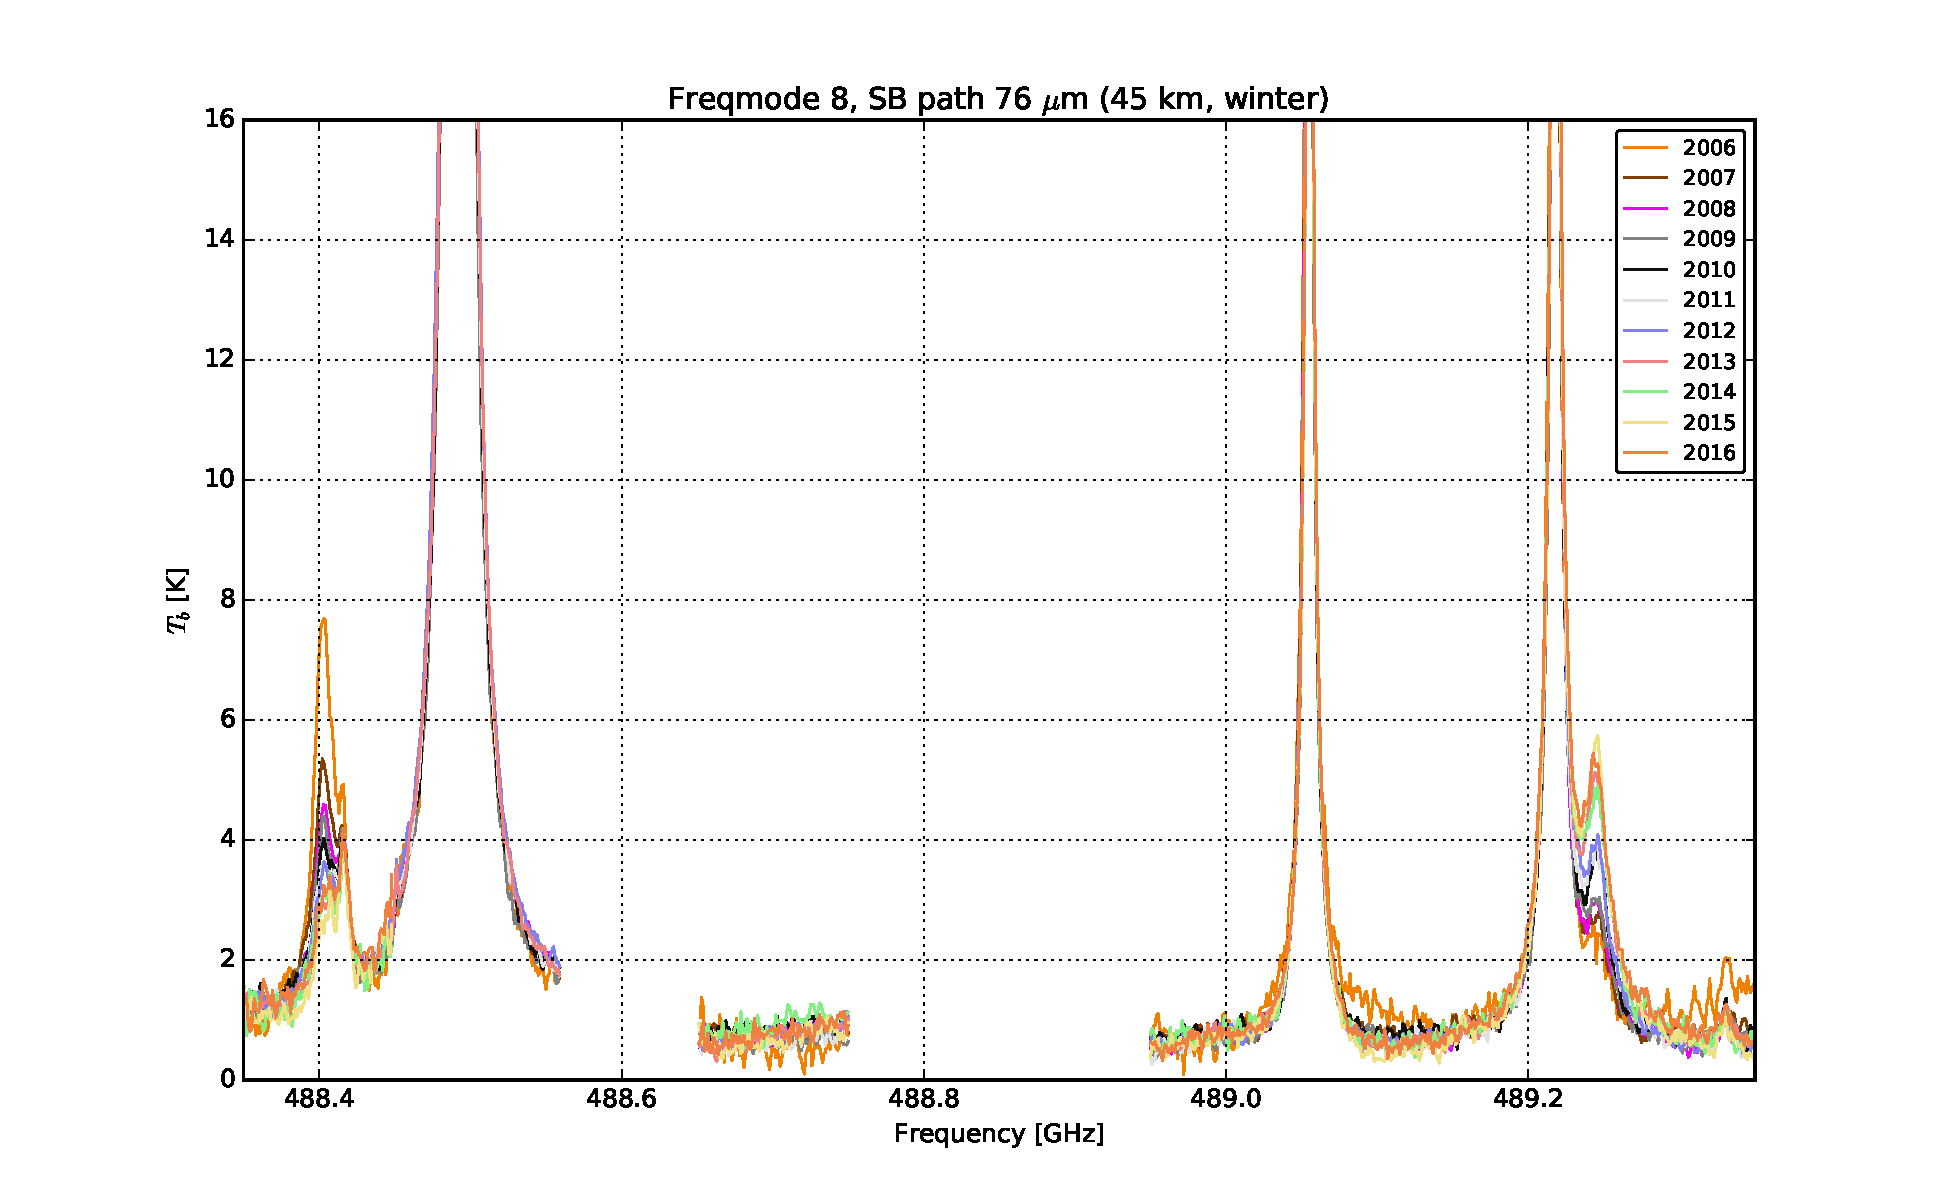
\includegraphics[width=\textwidth]{spectra/fm_08_spectra_winter_76u}
        \caption{winter}\label{fig:spectra:08:winter:76u}
    \end{subfigure}
    \caption{Annual median spectra for FM~08 for altitude interval 40--50~km at
        equatorial latitudes for the $76\,\mathrm{\mu m}$ sideband path. The
        unhealthy sub-bands~7 and~3 are between $\sim488.45$
        and~$488.65\,\mathrm{GHz}$.
        }\label{fig:spectra:08:76u}
\end{figure}

\begin{figure}[ht]
    \centering
    \begin{subfigure}[b]{0.9545\textwidth}
        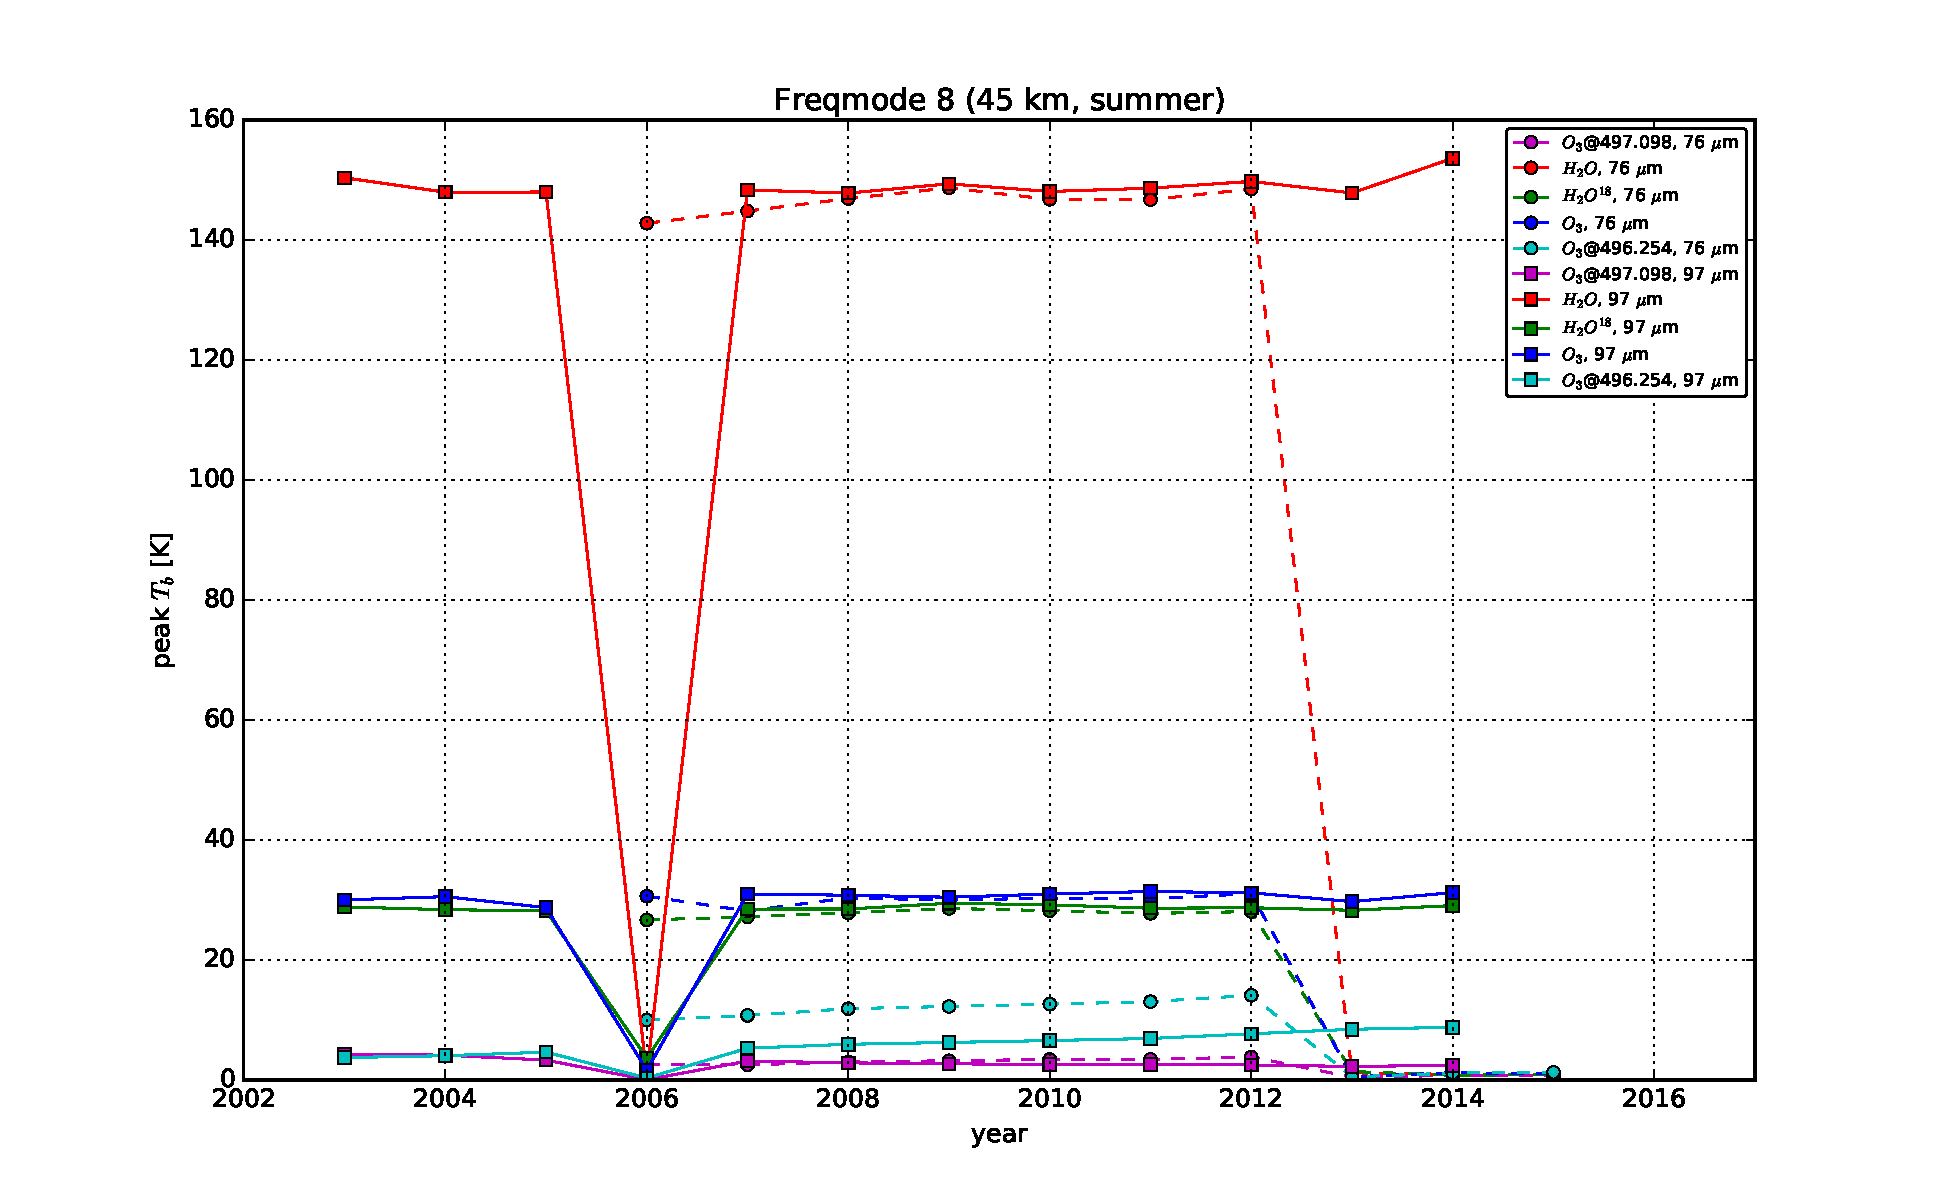
\includegraphics[width=\textwidth]{peaks/fm_08_peaks_summer}
        \caption{summer}\label{fig:peaks:08:summer}
    \end{subfigure}
    \begin{subfigure}[b]{0.9545\textwidth}
        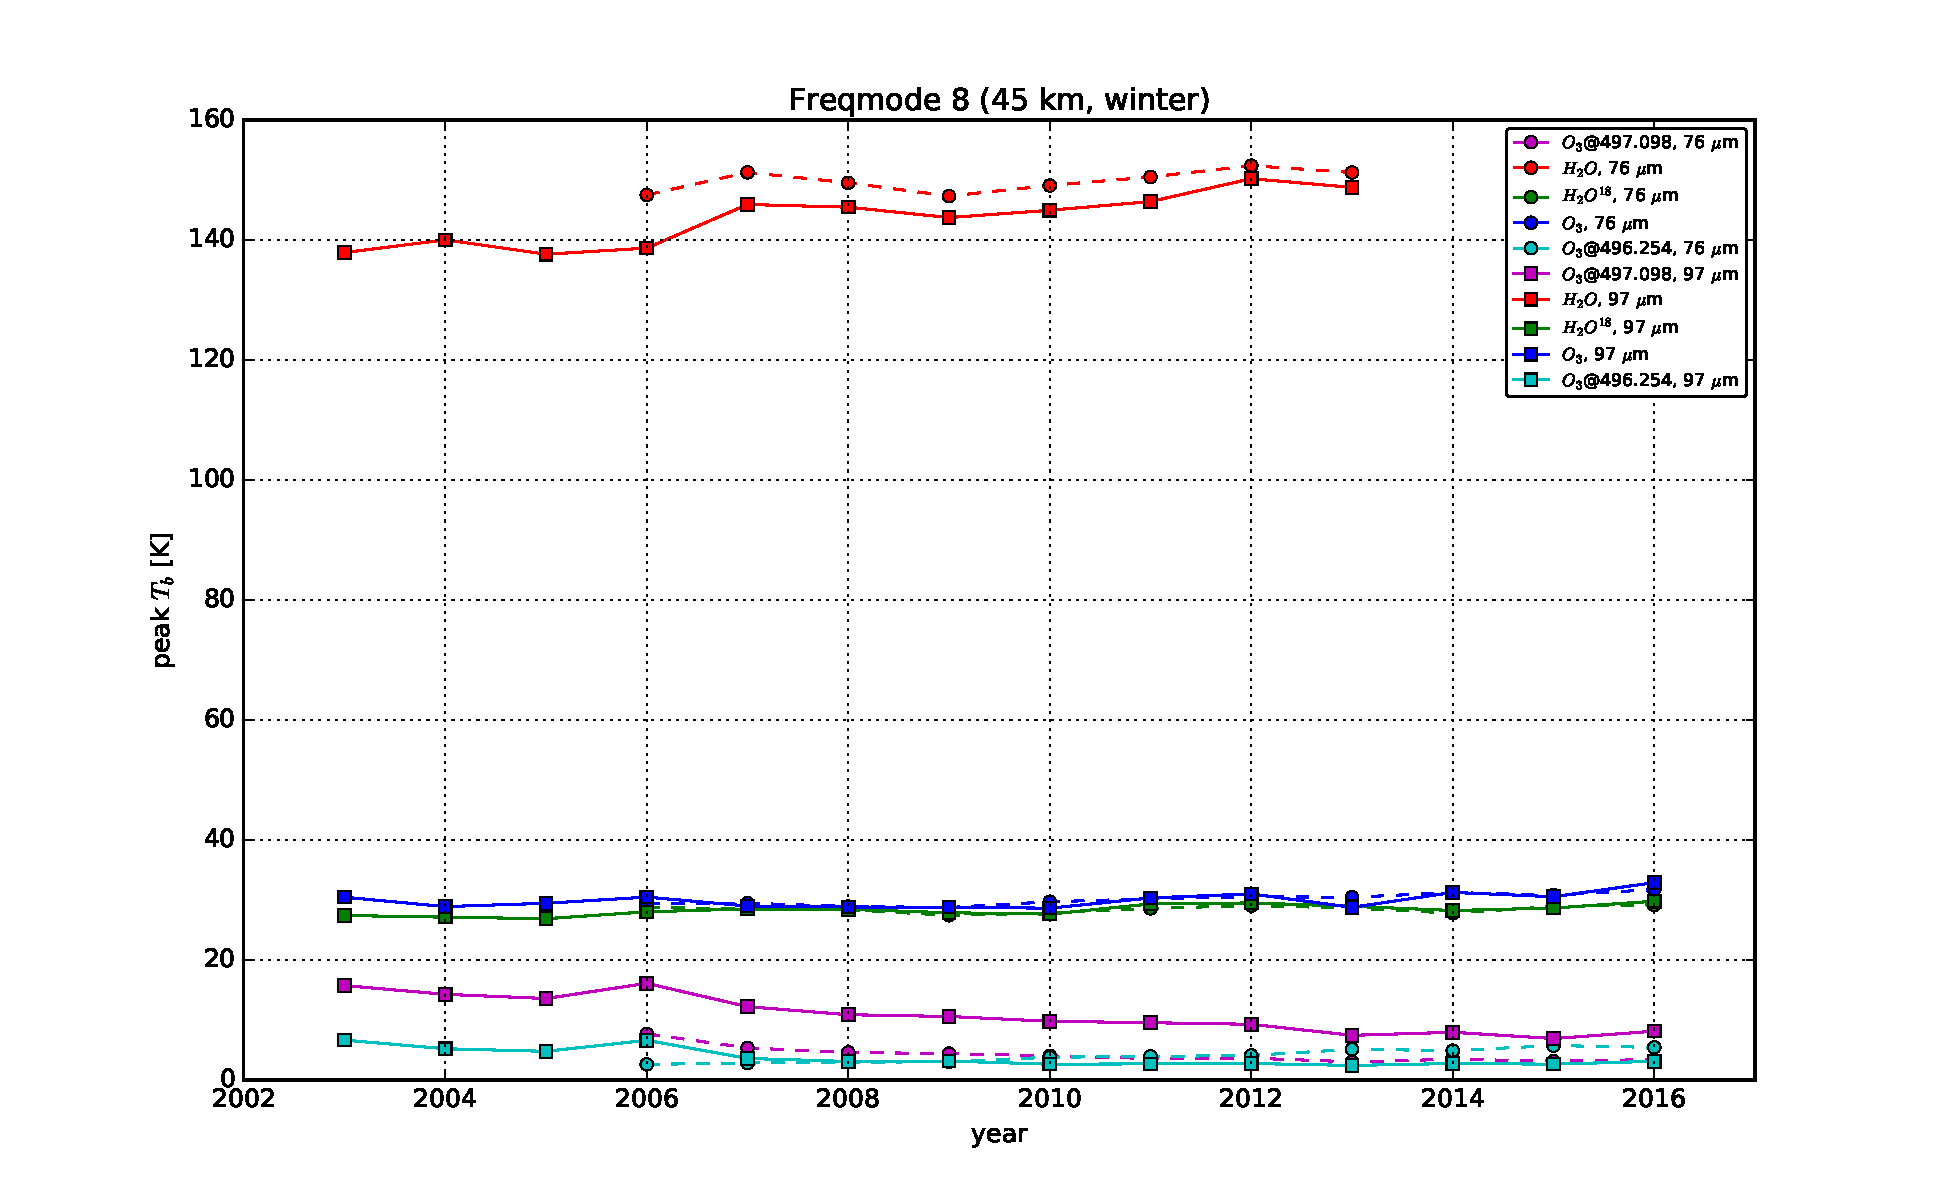
\includegraphics[width=\textwidth]{peaks/fm_08_peaks_winter}
        \caption{winter}\label{fig:peaks:08:winter}
    \end{subfigure}
    \caption{Annual median peak values for FM~08 for altitude interval
        40--50~km at equatorial latitudes for both sideband paths.
        Values extracted for the the \chem{H_2O} peak
        at~$\sim488.494\,\mathrm{GHz}$, the \chem{H_2O^{18}} peak
        at~$\sim489.055\,\mathrm{GHz}$, the \chem{O_3} peak
        at~$\sim489.218\,\mathrm{GHz}$, and the \chem{O_3} sideband peaks
        at~$\sim488.405$ and $\sim489.247\,\mathrm{GHz}$,
        in Figs.~\ref{fig:spectra:08:97u} and~\ref{fig:spectra:08:76u}.
        }\label{fig:peaks:08}
\end{figure}

\noindent
FM~08 is different from the other modes in two respects: first, it is a lower
sideband mode, which for the purpose of this report is not important; second,
it has utilised two separate sideband paths for most of its operation, that
show distictly different sideband leakage charateristics.  Yearly median
spectra for summer and winter at $\sim45\,\mathrm{km}$ are shown in
Figs.~\ref{fig:spectra:08:97u} and~\ref{fig:spectra:08:76u} for the two
sideband paths~$97$ and~$76\,\mathrm{\mu m}$ respectively, and the trend over
time of the different peaks can be seen in Fig.~\ref{fig:peaks:08}.

It is evident from the pictures that the sideband peaks (far left and far right
in the figures) have changed over the years, but the trends are different both
depending on which sideband path is looked at, and depending on the season.
These issues are discussed in greater detail in Sec.~\ref{FM08:sbl} below.
Apart from the sideband issues, and apart from a glitch in the summer of 2006
the spectra for the $97\,\mathrm{\mu m}$ path look good for both seasons.
Likewise, the spectra for the $76\,\mathrm{\mu m}$ also look good for both
seasons, apart from the summers of 2013--2016, in the last of which the this
path was not used at all.


\subsection{Sideband leakage}
\label{FM08:sbl}

\begin{figure}[ht]
    \centering
    \begin{subfigure}[b]{0.9545\textwidth}
        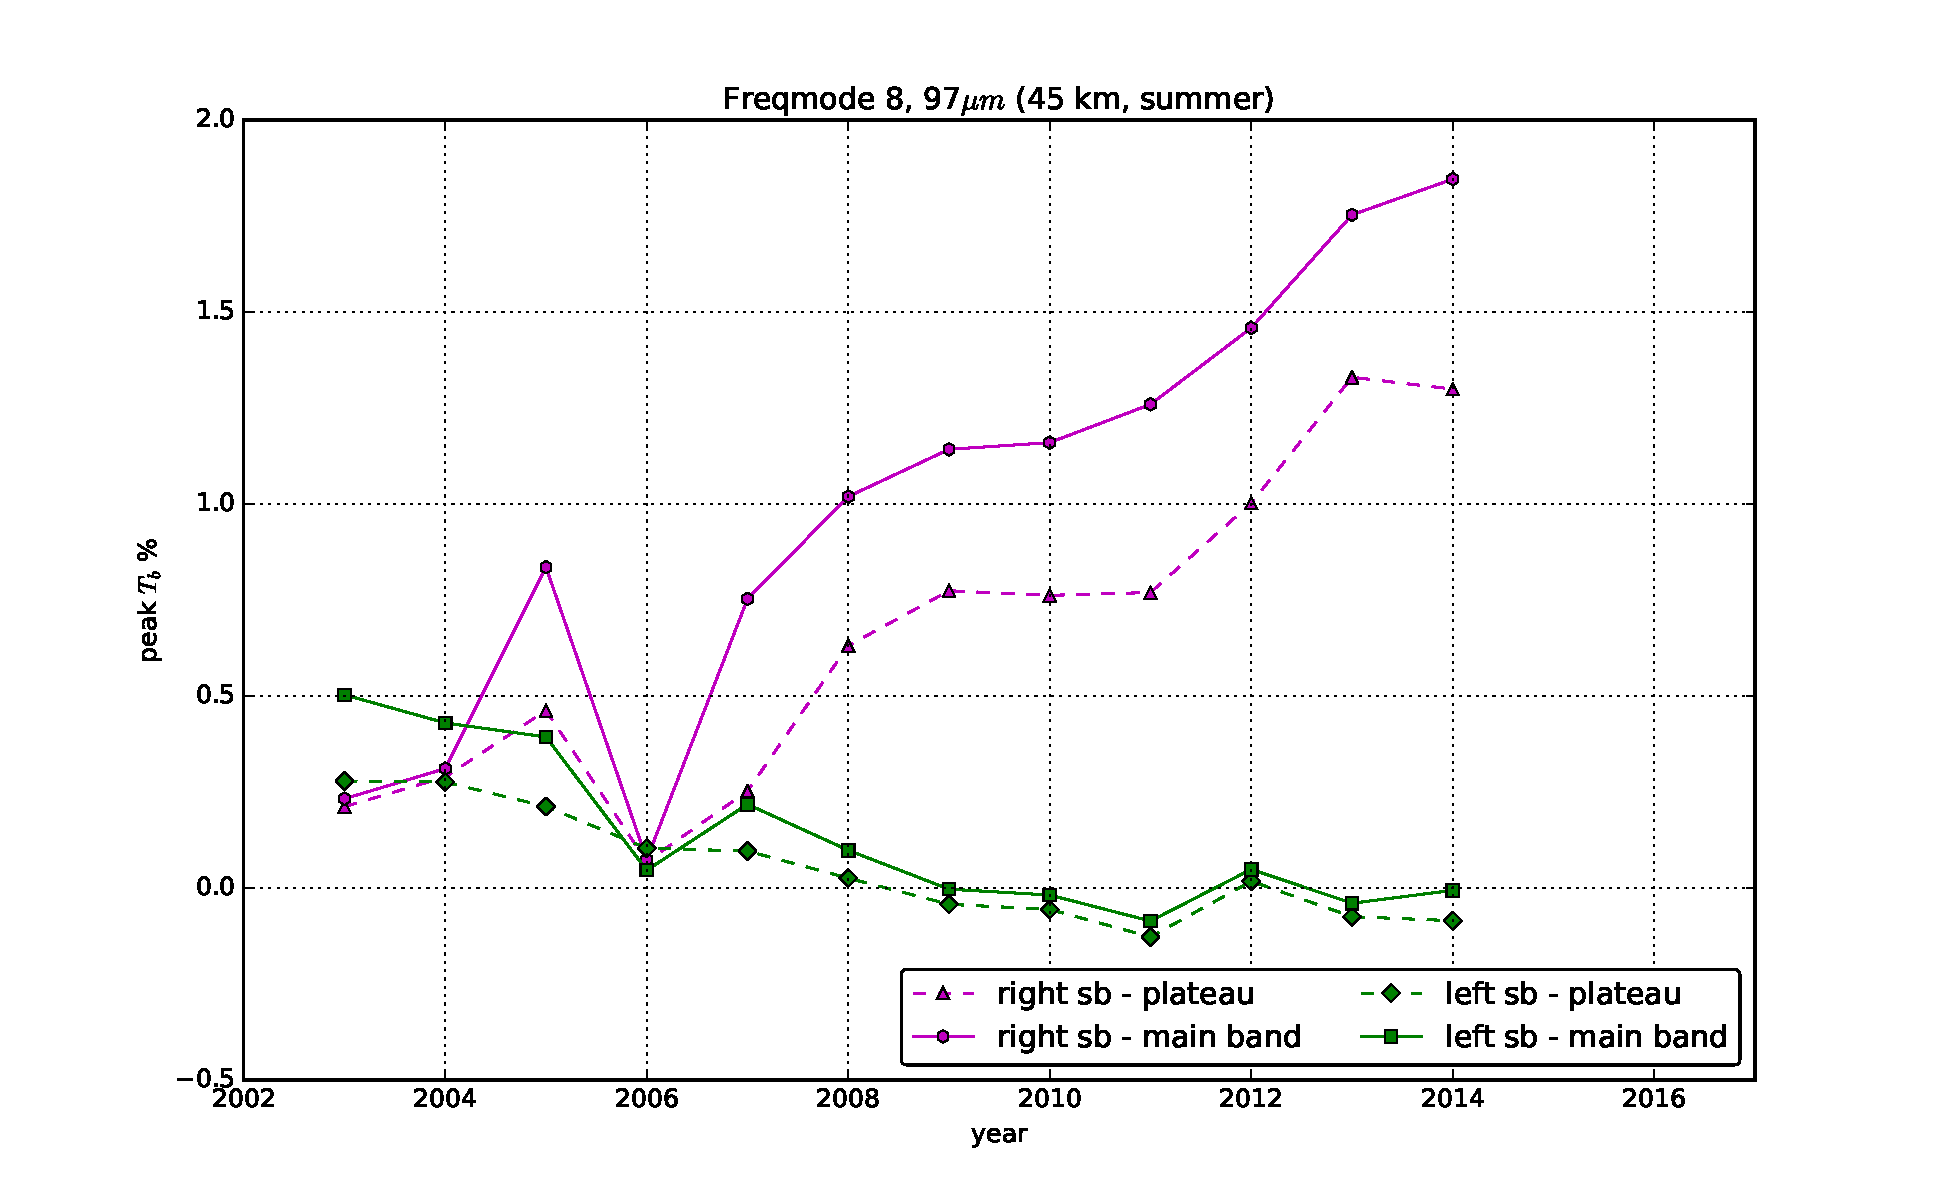
\includegraphics[width=\textwidth]{peaks/fm_08_sbl_summer_97u}
        \caption{summer}\label{fig:sbl:08:summer:97u}
    \end{subfigure}
    \begin{subfigure}[b]{0.9545\textwidth}
        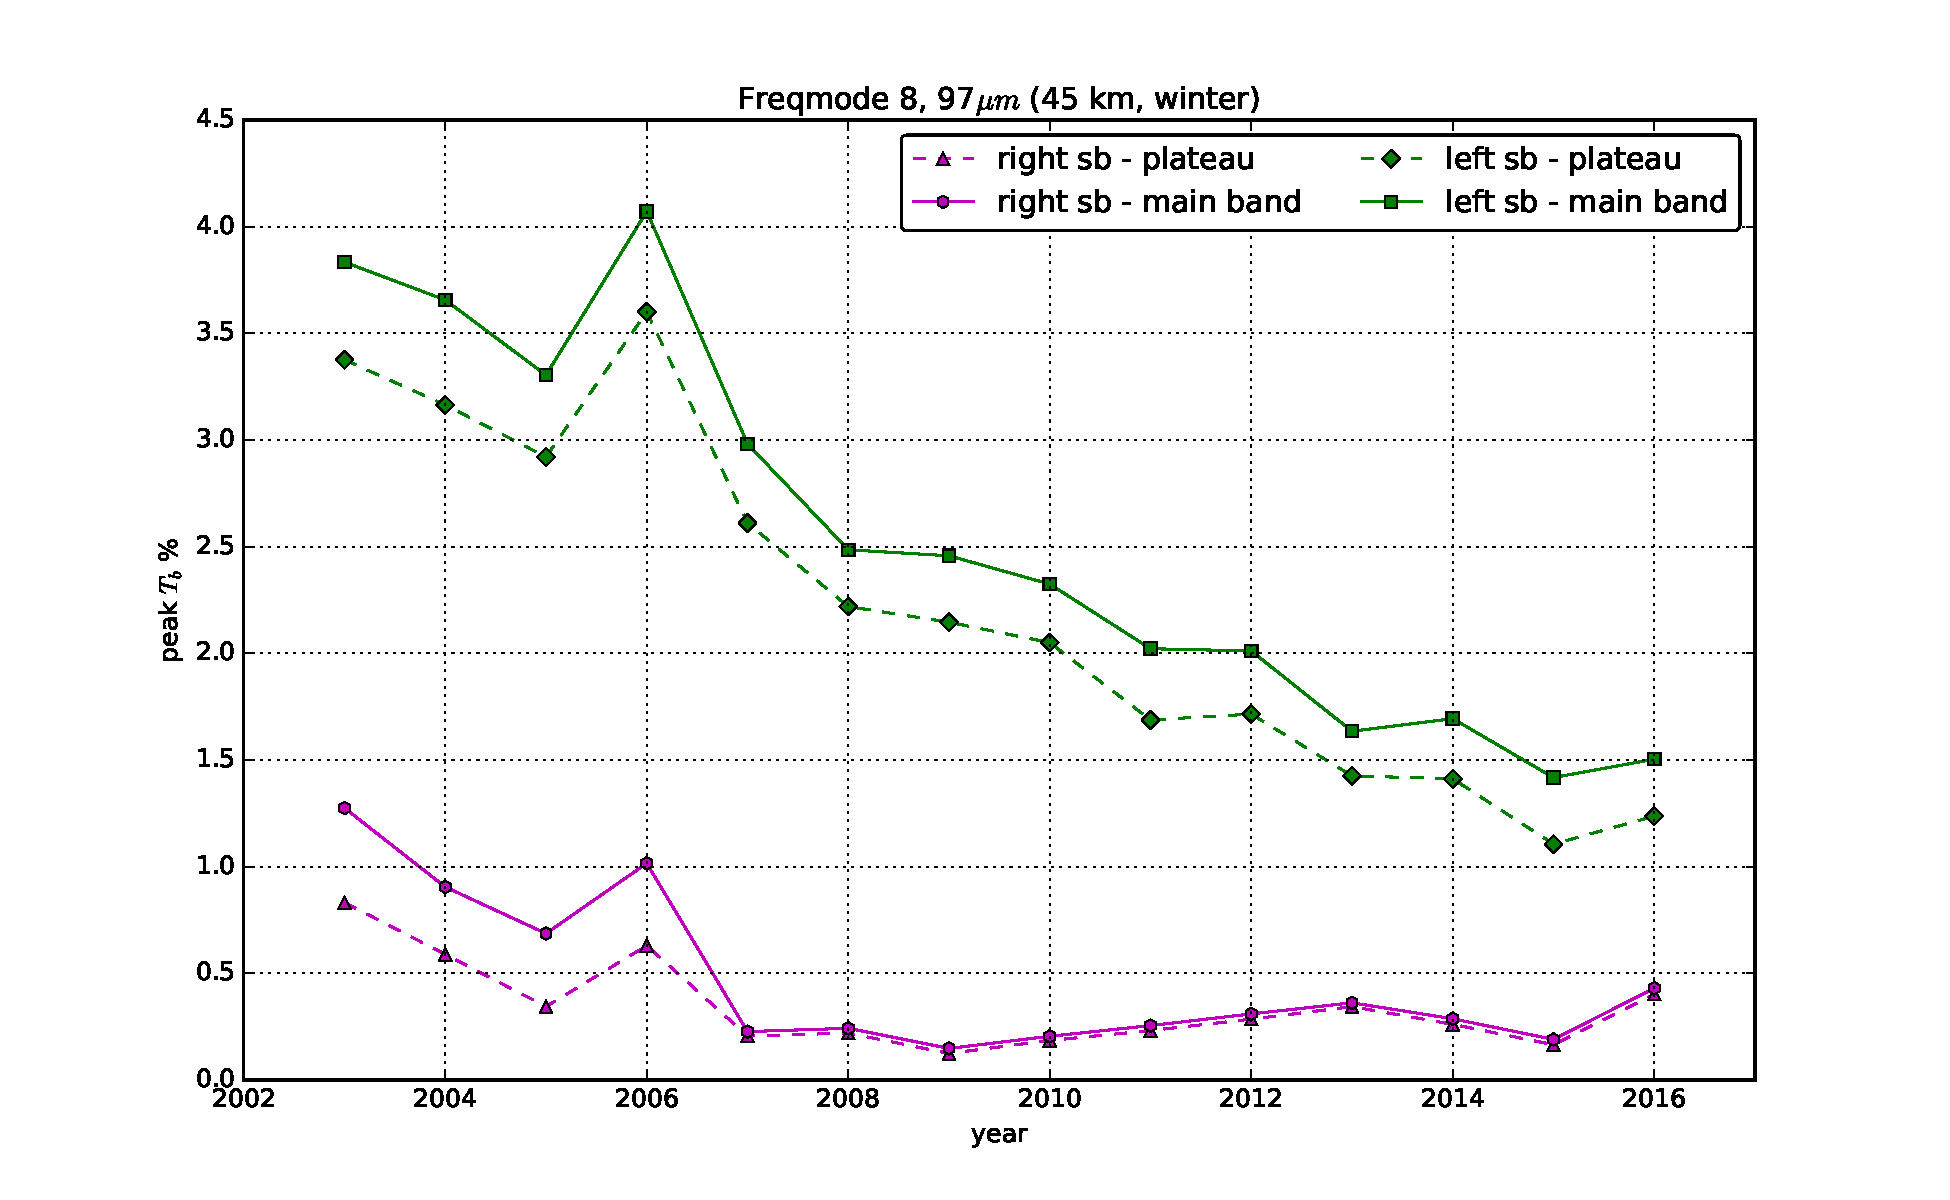
\includegraphics[width=\textwidth]{peaks/fm_08_sbl_winter_97u}
        \caption{winter}\label{fig:sbl:08:winter:97u}
    \end{subfigure}
    \caption{Sideband leakages in \% calculated from the data shown in
        Fig.~\ref{fig:spectra:08:97u} for the $97\,\mathrm{\mu m}$ sideband
        path.  Values were calculated by subtracting the value of the
        ``plateau'' on the side of each sideband peaks nearest its
        neighbouring mainband peak, or a first order approximation of the
        mainband value under the peak.  The results were compared with~$245.5$
        and~$256.8\,\mathrm{K}$ for the left and right sideband peaks
        respectively, values deemed representative of the actual peak
        intensities.
        }\label{fig:sbl:08:97u}
\end{figure}

\begin{figure}[ht]
    \centering
    \begin{subfigure}[b]{0.9545\textwidth}
        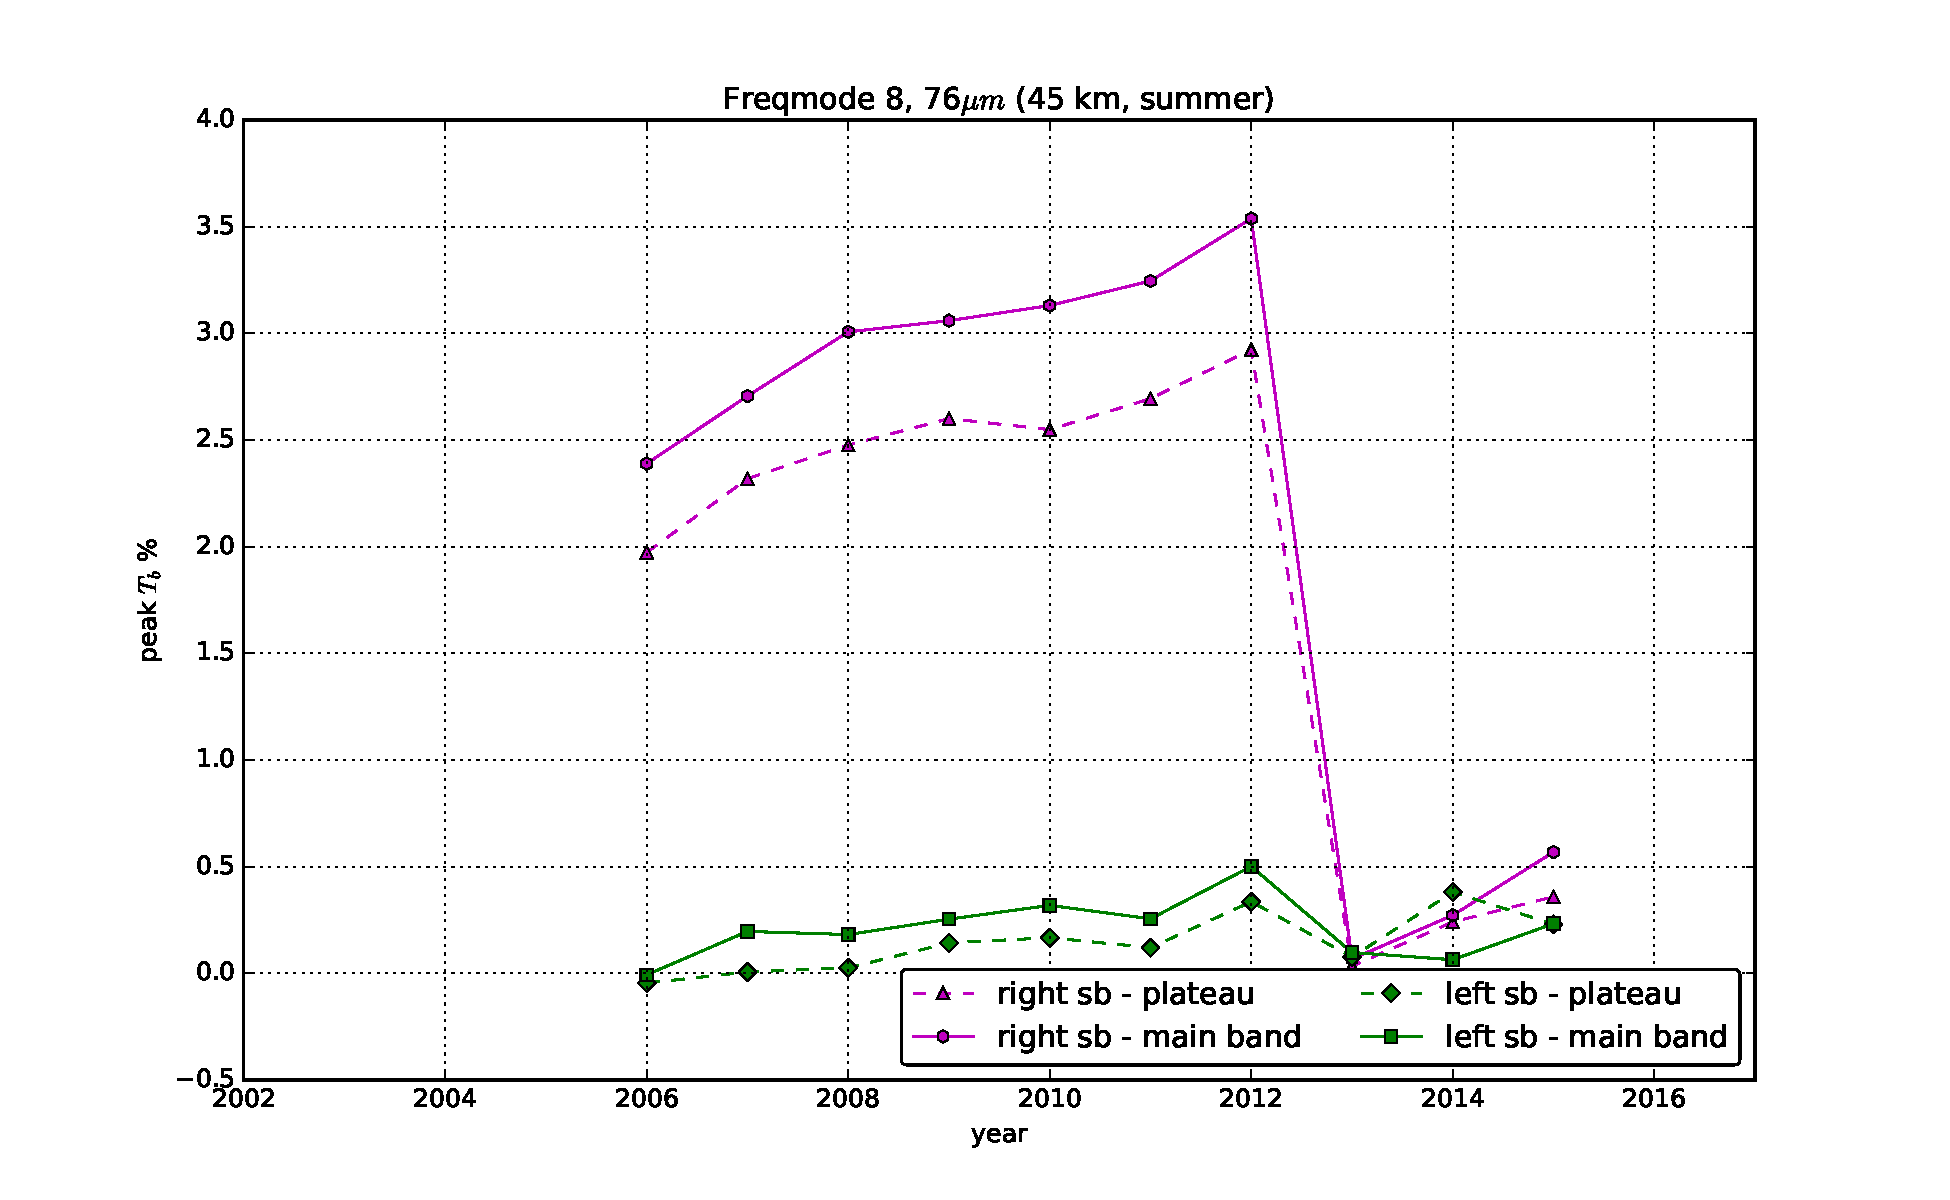
\includegraphics[width=\textwidth]{peaks/fm_08_sbl_summer_76u}
        \caption{summer}\label{fig:sbl:08:summer:76u}
    \end{subfigure}
    \begin{subfigure}[b]{0.9545\textwidth}
        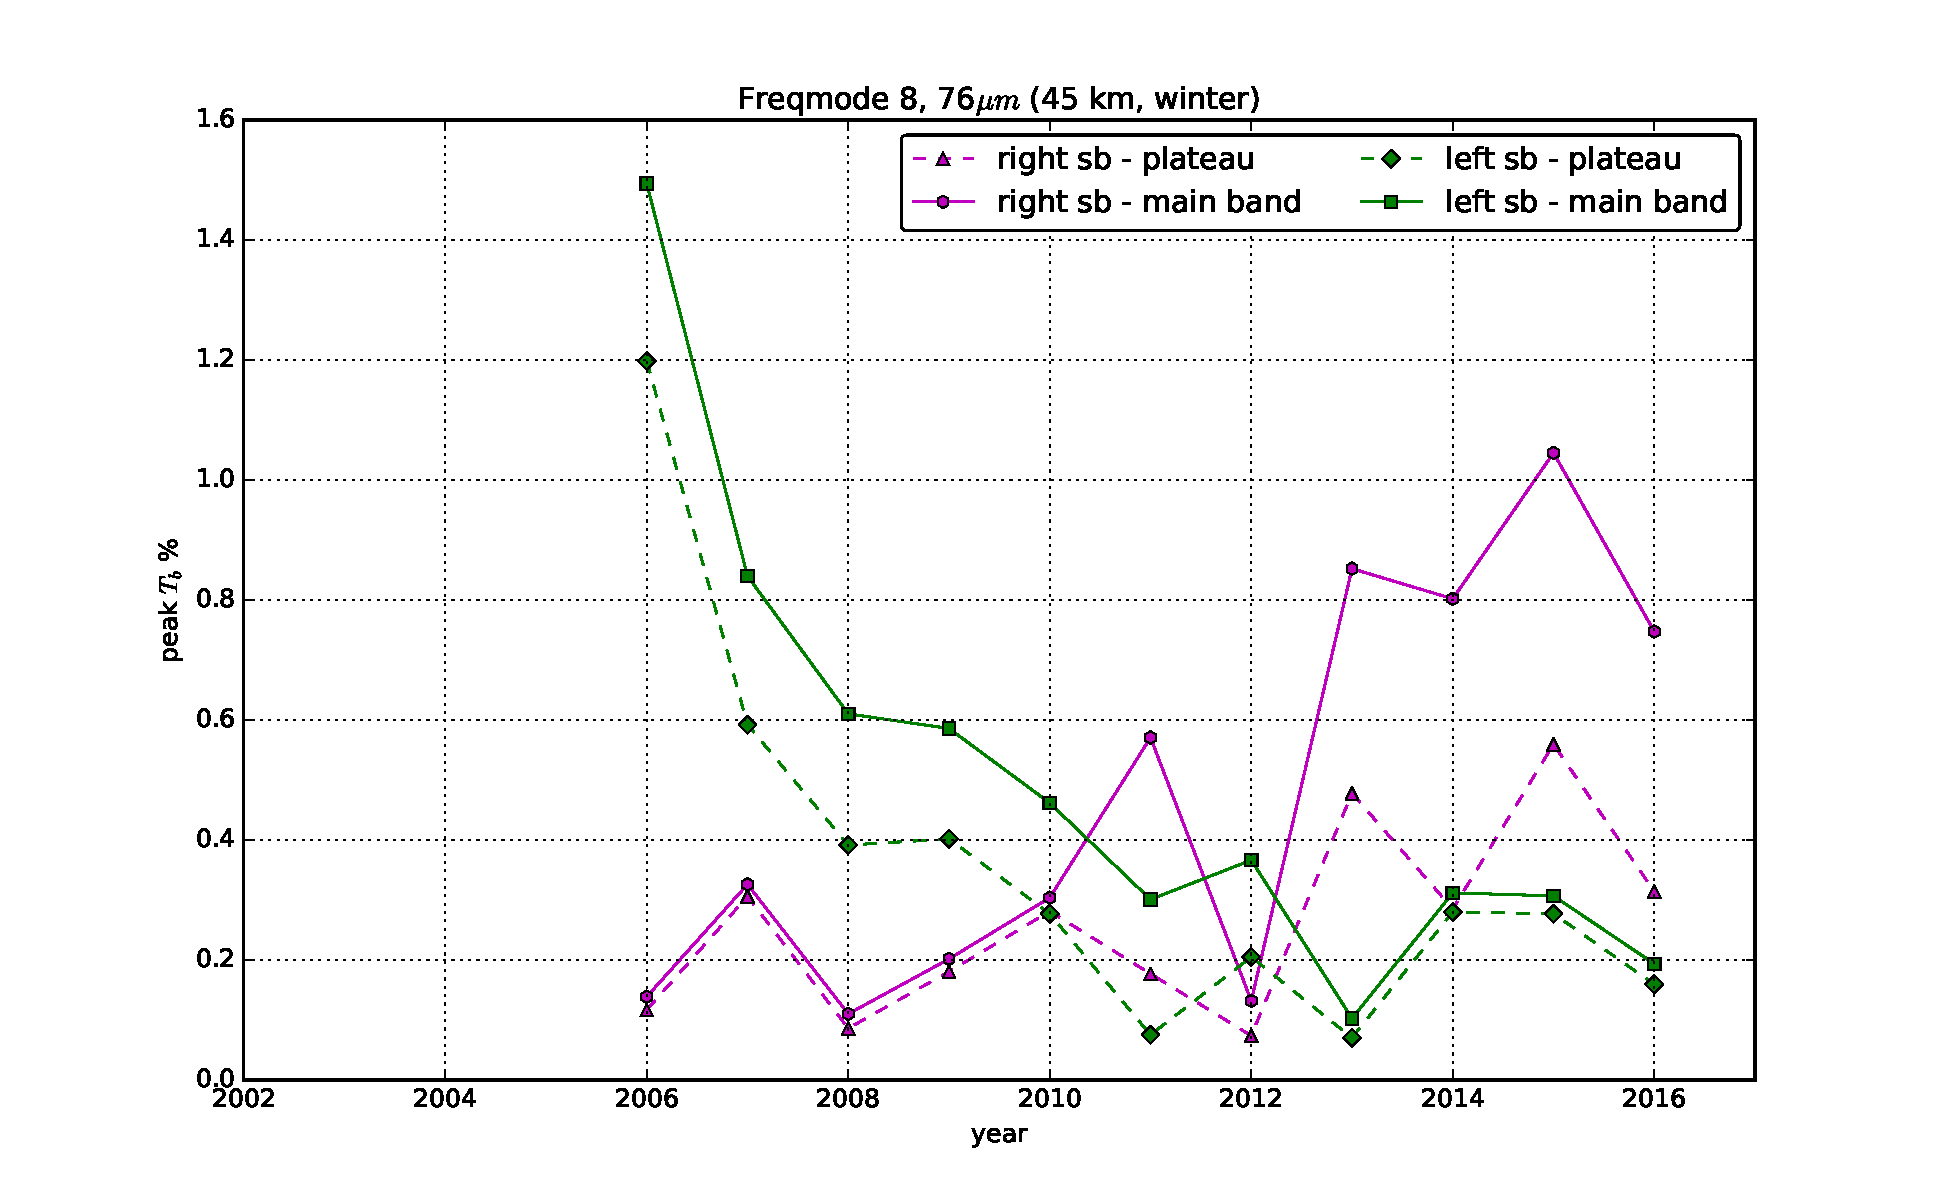
\includegraphics[width=\textwidth]{peaks/fm_08_sbl_winter_76u}
        \caption{winter}\label{fig:sbl:08:winter:76u}
    \end{subfigure}
    \caption{Sideband leakages in \% calculated from the data shown in
        Fig.~\ref{fig:spectra:08:76u} for the $76\,\mathrm{\mu m}$ sideband
        path.  Values were calculated by subtracting the value of the
        ``plateau'' on the side of each sideband peaks nearest its
        neighbouring mainband peak, or a first order approximation of the
        mainband value under the peak.  The results were compared with~$245.5$
        and~$256.8\,\mathrm{K}$ for the left and right sideband peaks
        respectively, values deemed representative of the actual peak
        intensities.
        }\label{fig:sbl:08:76u}
\end{figure}

\noindent


\subsubsection{Sideband paths}
\label{FM08:sbpath}
The sideband filter for FM~08 uses two more or less distinct values for the
sideband path length in equal measure: $97\,\mathrm{\mu m}$ and
$76\,\mu\mathrm{m}$.  The leakage tendency varies for the two categories,
\TODO{elaborate on sbpath for FM~08}


\subsection{Seasonality}
\label{FM08:seasonality}
\TODO{Add FM~08 seasonanlity elaboration}
